\section{Preliminaries}
\label{sec:prelim}

In this section we introduce notation and underlying assumptions (Section \ref{subsec:notation-assume}), 
and define our observability (Section \ref{subsec:observe}) and cross-validation (Section \ref{subsec:xval}) rules.

%Before starting our analysis, we detail the notation used in this document.

\subsection{System Assumptions, Notation and Terminology}
\label{subsec:notation-assume}

In this work, we make the following assumptions about PMU placements and buses:
\begin{enumerate}
	\item A PMU can only be placed on a bus.
	\item A PMU on a bus measures the voltage phasor at the bus and the current phasor of all transmission lines connected to it. 
	%\item A PMU on a bus measures the voltage phasor of the bus and the current phasor of all branches emerging from the bus.
	\item We assume all buses are zero-injection. A bus is zero-injection if it has no load nor generator \cite{Zhang10}.  Kirchhoff's Current Law can only be applied to zero-injection buses.
\end{enumerate}

We model a power grid as an undirected graph $G=(V,E)$.  Each $v \in V$ represents a bus.  A bus is either an electrical substation, a power generation center, or an 
aggregation of loads. Each $(u,v) \in E$ is a transmission line connecting buses $u$ and $v$.  Figure \ref{fig:example} is an example of a power system modeled as an undirected graph.

\begin{figure}[t]
\centering
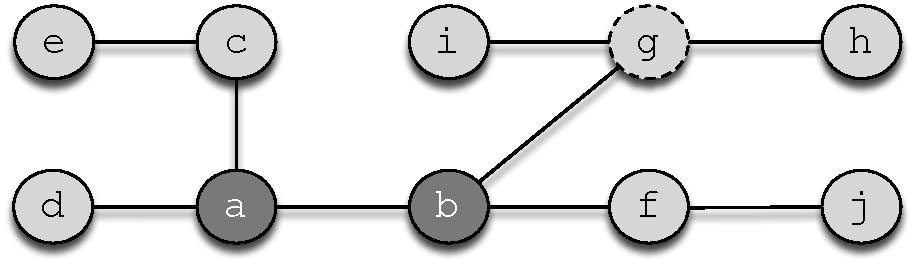
\includegraphics[scale=0.51]{figs/example4.pdf}
%\includegraphics[scale=0.51]{figs/example2.pdf}
\caption{Example power system graph. The dark shaded nodes -- $a$ and $b$ -- have PMUs.} 
\label{fig:example}
\end{figure}

Using the same notation as Brueni and Heath \cite{Brueni05}, we define two $\Gamma$ functions. For $v\in V$ let $\Gamma(v)$ be the set of $v$'s neighbors in $G$, and $\Gamma[v] = \Gamma(v)\cup \{v\}$.
A PMU placement $\Phi_G \subseteq V$ is a set of nodes at which PMUs are placed,
%We use the definition of a PMU placement from Brueni and Heath \cite{Brueni05}: a PMU cover, $\Phi$, is a subset of $V$ in which PMUs are placed such that all $v \in V$ and all $(u,v) \in E$ observed.
and $\Phi^R_G\subseteq V$ is the set of observed nodes for graph $G$ with placement $\Phi_G$ (see definition of observability below). %For convenience, we let $\Phi^R$ represent the observed nodes for graph $G$.
$k^* = \min \{|\Phi_G|:\Phi^R_G=V\}$ is used to denote the minimum number of PMUs needed to observe the entire network.
%Finally, $m$ is a constant corresponding to a graph $G=(V,E)$ such that $m < |V|$. 

%We let $\Phi^-$ represent the observed edges and $\Phi^R$ represent the observed nodes.
%All notation used in this document is shown in Table \ref{tab:notation}.

For convenience, we refer to any node with a PMU as a \emph{PMU node}. Additionally, we shall say that a set $W\subseteq V$ is observed if all nodes in the set are observed, and if $W=V$ we refer to the graph as \emph{fully observed}. 


%%%%%%%%%%%%%%%%%%%%%%%%%%%%%%%%%%%%%%%%%%%%%%%%%%%%%%%%%%%%%%%%%%%% BEGIN COMMENT %%%%%%%%%%%%%%%%%%%%%%%%%%%%%%%%%%%%%%%%%%%%%%%%%%%%%%%%%%%%%%%%%%%%%%%%%%%%%%%%%%%%%%%%%%%%%%%%%%%%%%%%%%%%%%%%
\begin{comment}
\begin{table}[t]
\begin{center}
\begin{tabular}{l l} 
\hline \hline
   	{\bf Notation} & {\bf Meaning} \\
		  \hline 
		  	$G$ &  undirected graph $(V,E)$ where each $v \in V$ is a bus and each \\
				&  $(u,v) \in E$ is a transmission line connecting $u$ and $v$\\
			$\Gamma(v)$ & $\{u \in V$ $|$ $(u,v) \in E \}$ \\ 
			$\Gamma[v]$ & $\Gamma(v) \cup \{v\}$ \\
 		 	$n$ & $|V|$ \\
			$\Phi$ & a subset of $V$ in which PMUs are placed such that all \\ 
				   & $v \in V$ and all $(u,v) \in E$ observed  \\
			$\Phi^R$ & set of observed nodes \\
			$\Phi^-$ & set of observed edges \\
			\hline \hline
	\end{tabular}
	\end{center}
\caption{Notation Table}
\label{tab:notation}
\end{table}
\end{comment}
%%%%%%%%%%%%%%%%%%%%%%%%%%%%%%%%%%%%%%%%%%%%%%%%%%%%%%%%%%%%%%%%%%%% END COMMENT %%%%%%%%%%%%%%%%%%%%%%%%%%%%%%%%%%%%%%%%%%%%%%%%%%%%%%%%%%%%%%%%%%%%%%%%%%%%%%%%%%%%%%%%%%%%%%%%%%%%%%%%%%%%%%%%

\subsection{Observability Rules}
\label{subsec:observe}

We use the simplified observability rules elegantly stated by Brueni and Heath \cite{Brueni05}. For completeness, we restate the rules here:
\begin{enumerate}
	
	\item {\bf Observability Rule 1 (O1)}.  {\it If  node $v$ is a PMU node, then $\Gamma[v]$ is observed. Formally, if $v \in \Phi$, then $\Gamma[v] \subseteq \Phi^R_G$. }

	\item {\bf Observability Rule 2 (O2)}. {\it If a node $v$ is observed and  $\Gamma(v)\backslash\{u\}$ is observed for some $u\in\Gamma(v)$, then  $\Gamma[v]$ is observed.
	Formally, if $v \in \Phi^R_G$ and $|\Gamma(v) \cap (V - \Phi^R_G)| \leq 1$, then $\Gamma[v] \subseteq \Phi^R_G$. }

\end{enumerate}

Consider the example in Figure \ref{fig:example}, where the shaded nodes are  PMU nodes.
Using O1, the PMU at $a$ results in the observation of $a$, $c$, and $d$. Likewise, the PMU at $b$ make $b$, $f$, and $e$ observed.
Finally, O2 can be applied at $e$ because $e$ is observed and all of $e$'s neighbors except $i$ are observed. As a result, $i$ becomes observed. 
Note that O2 cannot be applied at $f$ because $f$ has two unobserved neighbors. %This leaves $g$ and $h$ as the only two unobserved nodes in this example. 

%\begin{figure*}[t]
%  \begin{center}
%    \fbox{\subfigure[Case O1]{\label{fig:s1}\includegraphics[scale=0.28]{figs/s1.pdf}}}
%    \fbox{\subfigure[Case O2]{\label{fig:s2}\includegraphics[scale=0.28]{figs/s2.pdf}}} 
%  \end{center}
%	\caption{Rule Set 2} 
%  \label{fig:ruleset2}
%\end{figure*}




\subsection{Cross-Validation Rules}
\label{subsec:xval}

% If phasor measured by 2 or more PMUs
From Vanfretti et al. \cite{Vanfretti10}, PMU measurements can be cross-validated when: (1) a 
voltage phasor of a non-PMU bus can be computed by PMU data from two different buses or (2) the current phasor of a transmission line can be computed from PMU data from two different buses. 
%Note that Vanfretti et al. \cite{Vanfretti10} use the term ``redundancy'' instead of cross-validation.  
{\footnote {\small  Vanfretti et al. \cite{Vanfretti10} use the term ``redundancy'' instead of cross-validation. }}  
Although PMU data is actually being cross-validated,
for convenience, we say a PMU is cross-validated. Below is a precise statement of the cross-validation rules taken from  Vanfretti et al. \cite{Vanfretti10}. 
A PMU is \emph{cross-validated} if one of the rules below is satisfied: 
\begin{enumerate}
	
	\item {\bf Cross-Validation Rule 1 (XV1)}.  {\it Adjacent PMU nodes cross-validate each other. % (Figure \ref{fig:validate}(a)). 
	Formally, $u, v \in \Phi$, $u \in \Gamma(v)$, and $v \in \Gamma(u)$.}

	\item {\bf Cross-Validation Rule 2 (XV2)}. {\it PMU nodes with a common neighbor with no PMU cross-validate each other. % (Figure \ref{fig:validate}(b)). 
	Formally, $u, v \in \Phi$, $v \notin \Gamma(u)$, 
	$u \notin \Gamma(v)$ and $\exists w$ such that $v \neq w$, $u \neq w$, $w \in \Gamma(v)$, $w \in \Gamma(u)$, and $w \notin \Phi$.}
\end{enumerate}
In short, the cross-validation rules require that {\em the PMU is within two hops of another PMU}.
For example, in Figure \ref{fig:example}, the PMUs at $a$ and $b$ cross-validate each other by XV1. 
%because both PMUs directly measure the current phasor of transmission line $(a,b)$.  
%Thus, given $2$ PMUs this represents the optimal placement of PMUs: the PMUs are cross-validated and the maximum number of nodes are observed.

%\begin{figure}[t]
%  \begin{center}
%  	\mbox{
%    \fbox{\subfigure[Cross-Validation Rule 1]{\label{fig:validate2}\includegraphics[scale=0.51]{figs/xvalidate-2nodes.pdf}}}
%    \fbox{\subfigure[Cross-Validation Rule 2]{\label{fig:validate3}\includegraphics[scale=0.51]{figs/xvalidate-3nodes.pdf}}} 
%	}
%  \end{center}
%	\caption{Example to illustrate cross-validation rules. The blue nodes indicate nodes with a PMU.}
%  \label{fig:validate}
%\end{figure}



